%
% wavelet.tex
%
% (c) 2019 Prof Dr Andreas Müller, Hochschule Rapperswil
%
\section{Wavelets
\label{section:spline-wavelets}}
\rhead{Spline-Wavelet}
Die Funktionen $B_n$ erfüllen eine Skalierungsrelation, es besteht also
die Hoffnung, dass daraus eine Multiskalen-Analyse konstruiert werden kann.
Dazu muss zunächst die Fourier-Transformierte von $B_n$ bestimmt werden,
da alle Konstruktionen von Abschnitt~ \ref{section:skalfour} im
Frequenzbereich stattgefunden haben.
Anschliessend kann das Orthonormalisierungsverfahren von
Abschnitt~\ref{section:orthonormalisierung} auf die Funktionen $B_n$
angewendet werden.
Schliesslich kann man aus den Koeffizienten der Skalierungsrelation
auch die Koeffizienten des Wavelets ableiten und so das Wavelet
bestimmen.

\subsection{Fourier-Transformierte $\hat{B}_n$
\label{subsection:spline-ft}}
Die Fourier-Transformierte von $B_n$ kann dank der Faltungsformel für die
Fourier-Transfomierte 
\begin{equation}
\hat{B}_n = \widehat{B_0 * B_{n-1}} = \sqrt{2\pi}\hat{B}_0 \cdot \hat{B}_{n-1}
\qquad
\hat{B}_n = (\!\sqrt{2\pi})^n \hat{B}_0^{n-1}
\label{Bn-ft}
\end{equation}
berechnet werden.
Es muss also nur $\hat{B}_0$ berechnet werden.

Die Fourier-Transformierte von $B_0$ ist
\begin{align*}
\hat{B}_0(\omega)
&=
\frac1{\sqrt{2\pi}}
\int_{-\infty}^{\infty}
B_0(t) e^{-i\omega t}\,dt
=
\frac1{\sqrt{2\pi}}
\int_0^1 e^{-i\omega t}\,dt
=
\frac1{\sqrt{2\pi}}
\biggl[
\frac{1}{-i\omega} 
e^{-i\omega t}
\biggr]_0^1
\\
&=
\frac1{\sqrt{2\pi}}
\frac{e^{-i\omega}-1}{-i\omega}
=
\frac1{\sqrt{2\pi}}
\frac{1-e^{-i\omega}}{i\omega}
=
\frac1{\sqrt{2\pi}}
\frac{2}{\omega}
e^{-i\omega/2}
\frac{e^{i\omega/2} - e^{-i\omega/2}}{2i}
\\
&=
\frac1{\sqrt{2\pi}}
e^{-i\omega/2}
\frac{\displaystyle\sin\frac{\omega}2}{\displaystyle\frac{\omega}2}
=
\frac1{\sqrt{2\pi}}
e^{-i\omega/2}
\sinc\frac{\omega}2.
\end{align*}
Daraus und aus \eqref{Bn-ft} folgt jetzt der folgende Satz

\begin{satz}
\label{satz:Bn-ft}
Die Fourier-Transformierte von $B_n$ ist
\begin{align*}
\hat{B}_n(\omega)
&=
(\!\sqrt{2\pi})^n
\hat{B}_0(\omega)^{n+1}
=
(\!\sqrt{2\pi})^n
\biggl(
\frac{1}{\sqrt{2\pi}}
e^{-i\omega/2} \sinc\frac{\omega}2
\biggr)^{n+1}
=
\frac{1}{\sqrt{2\pi}}
\biggl(
e^{-i\omega/2} \sinc\frac{\omega}2
\biggr)^{n+1},
\\
\hat{B}_0(\omega)
&=
\frac{e^{-i(n+1)\omega/2}}{\sqrt{2\pi}}
.
\end{align*}
\end{satz}

\subsection{Orthonormalisierung
\label{subsection:spline-orthonormalisierung}}
In Abschnitt~\ref{section:orthonormalisierung} wurde gezeigt, wie 
erreicht werden kann, dass die Translate einer Funktion orthonormiert
sind.
Dieses Verfahren soll jetzt auf die Funktionen $B_n$ angewendet werden.
Es wurde gezeigt, dass dazu zunächst die periodisierte Funktion
\[
\Phi_n(\omega)
=
2\pi \mathcal{P}|\hat{B}_n|^2(\omega)
\]
bestimmt werden muss. 
Den Periodisierungs-Operator kann man direkt berechnen:
\begin{align}
\mathcal{P} |\hat{B}_n|^2(\omega)
&=
\sum_{l\in\mathbb Z} |\hat{B}_n(\omega + 2\pi l)|^2
=
\frac{1}{2\pi}
\sum_{l\in\mathbb Z}
\biggl|
e^{-i\omega/2 -il\pi}
\sinc\biggl(\frac{\omega}2+l\pi\biggr)^{n+1}
\biggr|^2
\notag
\\
&=
\frac{1}{2\pi}
\sum_{l\in\mathbb Z}
\biggl|
(-1)^l
e^{-i\omega/2}
\frac{\sin\frac{\omega}2 \cdot (-1)^l}{\frac{\omega}2 + l\pi}
\biggr|^{2n+2}
\notag
\\
&=
\frac{1}{2\pi}
\sum_{l\in\mathbb Z}
\biggl(
\frac{\sin\frac{\omega}2}{\frac{\omega}2 + l\pi}
\biggr)^{2n+2}
=
\frac{1}{2\pi}
\sin^{2n+2}\frac{\omega}2
\cdot
\sum_{l\in\mathbb Z}
\biggl(
\frac{1}{\frac{\omega}2 + l\pi}
\biggr)^{2n+2}
\notag
\\
\Rightarrow\quad
\Phi_n(\omega)
=
2\pi\mathcal{P}|\hat{B}_n|^2(\omega)
&=
\biggl|\sin\frac{\omega}2\biggr|^{2n+2}
\sum_{l\in\mathbb Z}
\frac{1}{(\omega/2 + l\pi)^{2n+2}}
.
\label{Phin:expression}
\end{align}
Die Umformung in der zweiten Zeile ist nur möglich, wenn $\omega$
kein ganzzahliges Vielfaches von $2\pi$ ist, daher ist auch
\eqref{Phin:expression} nur gültig für $\omega$, die keine ganzzahligen
Vielfachen von $2\pi$ sind.

Die Formel~\eqref{Phin:expression} funktioniert nicht mehr, wenn $\omega$
ein Vielfaches von $2\pi$ ist, da dann der Zähler verschwinden kann.
Sei also $\omega = 2\pi k$ mit $k\in\mathbb Z$.
Wir müssen die Funktion $\sinc$ auf den Argumenten
$\omega/2+l\pi$ auswerten.
Wegen $\omega/2 + l\pi=k\pi + l\pi = (k+l)\pi$ sind dies die ganzzahligen
Vielfachen von $\pi$, deren Sinus verschwindet.
Es gilt nämlich
\begin{align*}
\sinc (\pi k)
&=
\begin{cases}
\sin(k\pi)/k\pi&\qquad k\ne 0\\
\sinc(0)=1&\qquad k=0
\end{cases}
\\
&=
\delta_{0k}.
\end{align*}
Damit kann jetzt auch $\Phi_n(\omega)$ für ganzzahlige Vielfache von $2\pi$ 
berechnet werden:
\begin{align*}
\mathcal{P}|\hat{B}_n|^2(\omega)
&=
\mathcal{P}|\hat{B}_n|^2(2\pi k)
=
\mathcal{P}|\hat{B}_n|^2(0)
=
\sum_{l\in\mathbb Z} |\hat{B}_n(2\pi l)|^2
\\
&=
\frac1{2\pi}
\sum_{l\in\mathbb Z} |e^{-il\pi}\sinc(l\pi)|^{2n+2}
=
\frac1{2\pi}
\sum_{l\in\mathbb Z} \delta_{l0}
=
\frac1{2\pi}
\\
\Rightarrow\qquad
\Phi_n(\omega)
&=
\Phi_n(2\pi k)
=
\Phi_n(0)=1.
\end{align*}
Damit kann die Fourier-Transformierte $\hat{\varphi}_n(\omega)$ als
\[
\hat{\varphi}_n(\omega)
=
\frac{\hat{B}_n(\omega)}{\sqrt{\Phi_n(\omega)}}
=
\frac{1}{\sqrt{2\pi}}
\biggl(e^{-i\omega/2}\sinc\frac{\omega}2\biggr)^{n+1}
\]
geschrieben werden.

Als nächstes muss die Funktion $1/\sqrt{\Phi_n(\omega)}$ in eine komplexe
Fourier-Reihe entwickelt werden.
Da die Funktion $\sinc$ gerade ist, ist auch $\Phi_n(\omega)$ gerade.
Da $\Phi_n(\omega)$ gerade ist, muss dies auch mit einer reinen
Fourier-Kosinus-Reihe möglich sein.
Dies bedeutet, dass die Koeffizienten $c_k$ der komplexen Fourier-Reihe
von $1/\sqrt{\Phi_n(\omega)}$ reell sind und $c_k=c_{-k}$,
sie können mit 
der Formel
\begin{equation}
c_k = c_{-k}
=
\frac{1}{2\pi}
\int_{-\pi}^{\pi}
\frac{\cos(k\omega)}{\sqrt{\Phi_n(\omega)}}
\,d\omega
\label{sqrtPhincoef}
\end{equation}
berechnet werden.

Aus der Lösung von Aufgabe~\ref{aufgabe:orthonormalisierung} ist bekannt,
dass das gesuchte Wavelet mit Hilfe der Koeffizienten gebildet werden 
kann:
\[
\varphi_n(\omega)
=
\sum_{k\in\mathbb Z}
c_k B_n(t-k)
=
\sum_{k\in\mathbb Z}
c_k T_kB_n(t).
\]
Da die Funktionen $B_n$ stückweise Grad-$n$-polynomiell sind, ist auch
$\varphi_n(\omega)$ stückweise Grad-$n$-polynomiell.

In \cite{buch:blatter} wird sogar gezeigt, dass $\sqrt{\Phi_n(\omega)}$
als Polynom in $\cos\omega$ mit rationalen Koeffizienten geschrieben
werden kann.
Wir benötigen diese Eigenschaft im folgenden nicht und sie ist auch nicht
weiter hilfreich für die Berechnung der Koeffizienten $c_k$, die mit
Hilfe der Formel \eqref{sqrtPhincoef}
numerisch berechnet werden müssen.

\begin{table}
\centering
\begin{tabular}{|>{$}c<{$}|>{$}r<{$}||>{$}c<{$}|>{$}r<{$}|}
\hline
 k&c_k&k&c_k\\
\hline
 0& 1.291394&16&-0.000282\\
 1&-0.174099&17& 0.000564\\
 2& 0.034928&18&-0.000282\\
 3&-0.007311&19& 0.000564\\
 4& 0.001566&20&-0.000282\\
 5& 0.000118&21& 0.000564\\
 6&-0.000172&22&-0.000282\\
 7& 0.000537&23& 0.000564\\
 8&-0.000275&24&-0.000282\\
 9& 0.000562&25& 0.000564\\
10&-0.000281&26&-0.000282\\
11& 0.000564&27& 0.000564\\
12&-0.000282&28&-0.000282\\
13& 0.000564&29& 0.000564\\
14&-0.000282&30&-0.000282\\
15& 0.000564&31& 0.000564\\
\hline
\end{tabular}
\caption{Koeffizienten des Vater-Wavelets für das Spline-Wavelet mit
$n=1$, also für ein stückweise lineares Wavelet.
Das zugehörige Vater-Wavelet ist in Abbildung~\ref{phi1:polygonzug}
dargestellt.
\label{table:B1-koef}}
\end{table}

\begin{beispiel}
Die numerische Berechnung der Koeffizienten $c_k$ für das Spline-Wavelet 
mit $n=1$ ergibt die Koeffizienten in Tabelle~\ref{table:B1-koef}.
Da die Funktion $\varphi_n(\omega)$ stückweise linear ist, muss man nur die
Werte für ganzzahliges $\omega$ berechnen könne, dazwischen ist
$\varphi_n(\omega)$ eine lineare Funktion.
Für $B_1$ gilt aber
\begin{align*}
B_1(k)
&=
\begin{cases}
1&\qquad k=1\\
0&\qquad 1\ne k\in\mathbb Z.
\end{cases}
\\
&=\delta_{1k}
\end{align*}
Für die Linearkombination $\varphi_n(k)$ gilt daher
\[
\varphi_1(k)
=
\sum_{l\in\mathbb Z} c_l B_1(k-l)
=
\sum_{k\in\mathbb Z} c_l \delta_{1,k-l}
=
c_{k-1}.
\]
Die Koeffizienten $c_k$ sind also im Wesentlichen die Funktionswerte
$\varphi_1(k)$.
Damit lässt sich der Graph von $\varphi_1$ als Polygonzug mit den Eckpunkten
$(k,c_{k-1})$ zeichnen, wie dies in Abbildung~\ref{phi1:polygonzug}
durchgeführt ist.
\begin{figure}
\centering
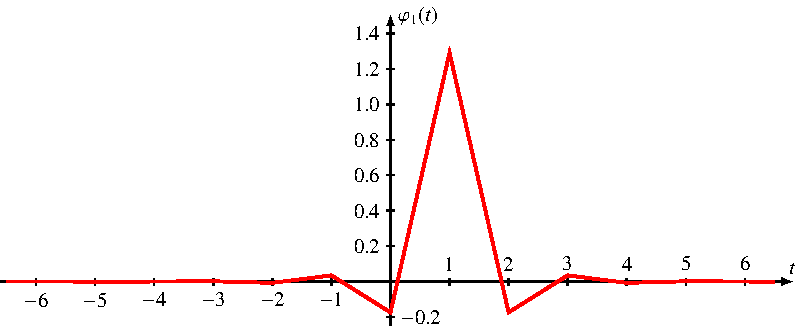
\includegraphics{chapters/9-spline/images/Bphi1.pdf}
\caption{Der Graph des stückweise linearen Vaterwavelets $\varphi_1$
ist ein Polygonzug mit den Ecken $(k,c_{k-1})$.
Die Koeffizienten $c_k$ sind in Tabelle~\ref{table:B1-koef} 
zusammengestellt.
\label{phi1:polygonzug}}
\end{figure}
\end{beispiel}

\subsection{Koeffizienten der Skalierungsrelation
\label{subsection:spline-skalierungskoeffizienten}}
Für die praktische Durchführung der Wavelet-Analyse mit Hilfe der
zugehörigen Multiskalen-Analyse brauchen wir die Skalierungsrelation 
für die Funktionen $\phi_n$ und daraus abgeleitet die
Skalierungsrelation für das zugehörige Wavelet $\psi_n$.

Da wir einen expliziten Ausdruck für die $\hat{\varphi}(\omega)$ haben,
können wir die Skalierungsrelation für $\varphi_n$ daraus ableiten.
Wir bezeichnen die erzeugende Funktion von $\varphi_n$ mit $H_n$.
Dann gilt
\begin{equation}
\begin{aligned}
\hat{\varphi}_n(\omega)
&=
H_n\biggl(\frac{\omega}2\biggr)
\,
\hat{\varphi}_n\biggl(\frac{\omega}2\biggr)
&&\Rightarrow&
H_n(\omega)
&=
\frac{\hat{\varphi}_n(2\omega)}{\hat{\varphi}_n(\omega)}
\end{aligned}
\label{Hnformel}
\end{equation}
Für die Fourier-Transformierte $\hat{\varphi}_n(\omega)$ haben wir früher
\[
\hat{\varphi}_n(\omega)
=
\frac{\hat{B}_n(\omega)}{\sqrt{\Phi_n(\omega)}}
\]
erhalten.
Setzen wir dies in \eqref{Hnformel} ein, erhalten wir
\begin{equation}
H_n(\omega)
=
\frac{\hat{B}_n(2\omega)}{\hat{B}_n(\omega)}
\frac{\sqrt{\Phi_n(\omega)}}{\sqrt{\Phi_n(2\omega)}}
\label{formel:phinskal}
\end{equation}

In Abschnitt~\ref{subsection:skalierungsrelation-phin} haben wir bereits
die Skalierungsrelation für die Spline-Funktionen $B_n$ gefunden und die
zugehörige erzeugende Funktion
\[
\tilde{H}_n(\omega) = \biggl(\frac{1+e^{-i\omega}}{2}\biggr)^{n+1}
\]
bestimmt.
Im Frequenzbereich ist die Skalierungsrelation für $\hat{B}_n(\omega)$
\[
\hat{B}_n(2\omega)=\tilde{H}_n(\omega) \, \hat{B}_n(\omega)
\qquad\Rightarrow\qquad
\frac{\hat{B}_n(2\omega)}{\hat{B}_n(\omega)}
=
\tilde{H}_n(\omega).
\]
Eingesetzt in \eqref{formel:phinskal} erhalten wir damit für die 
erzeugende Funktion 
\begin{equation}
H_n(\omega)
=
\tilde{H}_n(\omega)
\frac{\sqrt{\Phi_n(\omega)}}{\sqrt{\Phi_n(2\omega)}}
=
\biggl(
\frac{1+e^{-i\omega}}{2}
\biggr)^{n+1}
\frac{\sqrt{\Phi_n(\omega)}}{\sqrt{\Phi_n(2\omega)}}
\end{equation}

\subsection{Spline-Wavelet
\label{subsection:spline-wavelet}}





